IRSTI 50.47.00

\sectionwithauthors{A.D.Tulegulov , K.M. Akishev, D.S.Zhamangarin, B.O.Sataev}{THE USE OF DIGITAL TECHNOLOGIES FOR INTELLIGENT TRAFFIC MANAGEMENT}

\begin{center}
{\bfseries A.D.Tulegulov , K.M. Akishev, D.S.Zhamangarin, B.O.Sataev}

K. Kulazhanov Kazakh University of Technology and Business,

Astana, Kazakhstan,

е-mail: tad62@ya.ru
\end{center}

The purpose of the study is to develop, with the help of artificial
intelligence, an innovative digital microcontroller network traffic
light object capable of adaptively responding to traffic congestion and
changing the time phases of enabling the green signal in interaction
with neighboring traffic light objects.

The study uses a method of system analysis using computer simulation of
existing analog and hybrid traffic light controllers. As a result of the
study, an assessment of their effectiveness in the adaptive regulation
of modern traffic flows in densely populated cities of the country is
given. The results of simulation modeling in the AnyLogic PLE
environment were used for calculations. The experimental data of complex
entrance/exit road junctions of Almaty and Astana cities were taken as a
basis, taking into account the time cyclograms of traffic flow
characteristics of highways. An assessment was also given of the
existing methods of regulating complex road transport hubs to streamline
negative congestion in the center of Almaty and its expressways.

{\bfseries Keywords:} digital technologies{\bfseries ,} information systems,
artificial intelligence, machine vision, microcontroller, system
analysis, simulation modeling.

\begin{center}
{\large\bfseries КӨЛІК АҒЫНДАРЫН ИНТЕЛЛЕКТУАЛДЫ БАСҚАРУ ҮШІН ЦИФРЛЫҚ
ТЕХНОЛОГИЯЛАРДЫ ПАЙДАЛАНУ}

{\bfseries А.Д. Тулегулов,К.М. Акишев, Д.С. Жамангарин, Б.О. Сатаев}

Қ. Құлажанов атындағы Қазақ технология және бизнес университеті,

Астана, Қазақстан,

е-mail: tad62@ya.ru
\end{center}

Зерттеудің мақсаты-жасанды интеллект көмегімен қиылыстың жүктемесіне
бейімделе жауап беруге және көршілес бағдаршам нысандарымен өзара
әрекеттесу кезінде рұқсат етілген жасыл сигналды қосудың уақытша
фазаларын өзгертуге қабілетті инновациялық цифрлық микроконтроллерлік
желілік бағдаршам объектісін әзірлеу.

Зерттеу қолданыстағы аналогтық және гибридті бағдаршам контроллерлерін
компьютерлік модельдеуді қолдана отырып, жүйелік талдау әдісін қолданды.
Зерттеу нәтижесінде елдің халқы тығыз орналасқан қалаларының қазіргі
заманғы көлік ағындарын бейімделіп реттеудегі олардың тиімділігіне баға
берілді. Есептеулер жүргізу үшін AnyLogic ple ортасында Имитациялық
модельдеу нәтижелері пайдаланылды. Магистральдардың көліктік ағындық
сипаттамаларының уақытша циклограммаларын ескере отырып, Алматы және
Астана қалаларының күрделі кіру/шығу автокөлік тораптарының тәжірибелік
деректері негізге алынды. Сондай-ақ Алматы қаласының орталығында және
оның жүрдек магистральдарында жағымсыз кептеліс құбылыстарын ретке
келтіру үшін күрделі автокөлік тораптарын реттеудің қолданыстағы
әдістеріне баға берілді.

{\bfseries Түйін сөздер:} сандық технологиялар, ақпараттық жүйелер, жасанды
интеллект, машиналық көру, микроконтроллер, жүйелік талдау, Имитациялық
модельдеу.

\begin{center}
{\large\bfseries ПРИМЕНЕНИЕ ЦИФРОВЫХ ТЕХНОЛОГИЙ ДЛЯ ИНТЕЛЛЕКТУАЛЬНОГО УПРАВЛЕНИЯ
ТРАНСПОРТНЫМИ ПОТОКАМИ}

{\bfseries А.Д.Тулегулов,К.М. Акишев, Д.С. Жамангарин, Б.О.Сатаев}

Казахский университет технологии и бизнеса имени К. Кулажанова,

Астана, Казахстан,

е-mail: tad62@ya.ru
\end{center}

Цель исследования состоит в разработке с помощью искусственного
интеллекта инновационного цифрового микроконтроллерного сетевого
светофорного объекта, способного адаптивно реагировать на загруженность
перекрестка и менять временные фазы включения разрешающего зеленного
сигнала во взаимодействии с соседними светофорными объектами.

В исследовании использован метод системного анализа с использованием
компьютерного имитационного моделирования существующих аналоговых и
гибридных светофорных контроллеров. В результате исследования дана
оценка их эффективности в адаптивном регулировании современных
транспортных потоков густонаселенных городов страны. Для проведения
расчетов были использованы результаты имитационного моделирования в
среде AnyLogic PLE. За основу были взяты экспериментальные данные
сложных въездных/выездных автотранспортных узлов городов Алматы и Астана
с учетом временных циклограмм транспортных потоковых характеристик
магистралей. Также была дана оценка существующих методов регулирования
сложных автотранспортных узлов для упорядочения негативных заторных
явлений в центре города Алматы и его скоростных магистралях.

{\bfseries Ключевые слова:} цифровые технологии, информационные системы,
искусственный интеллект, машинное зрение, микроконтроллер, системный
анализ, имитационное моделирование.

\begin{multicols}{2}
{\bfseries Introduction}. The global experience in the development
of modern digital technologies for information exchange and the use of
intelligent control systems in the automotive industry has led to a
significant change in scientific, technological and practical approaches
to organizing optimal traffic in densely populated cities {[}1{]}.

The relevance of the study is due to an increase in the volume of
traffic flows both in large metropolitan areas and in small towns. The
existing mathematical models of traffic flow management are based on a
deterministic basis, in the differential equations of which the initial
and boundary conditions are empirically set, in which the relationship
between the definition of traffic flow and maximum load bandwidth is
contradictory. This leads to insufficient vehicle capacity during the
``peak hours'' of one of the traffic lanes with a significant load of
oncoming traffic lanes. In some developed countries, the idea of reverse
traffic is used, which requires a clear use of the administrative
resource of the traffic police and high discipline of motorists. Traffic
flow management has been widely used in the past.

The feasibility of the development is related to the need to optimize
traffic flows. Accidents, repairs, irrigation and utilities that are
unpredictable in time and space create additional resistance to traffic
flow, which is called a ``shock wave'' of congestion. As a result, the
capacity of the highway begins to decrease sharply, and traffic jams
occur.

From the point of view of hydrodynamics, the formation of additional
resistance leads to incomplete organization of flow movement. Such a
movement is called turbulent. His behavior is often difficult to
describe mathematically. It is known from hydraulics that the flow in
various coarse pipes is calculated on a semi-empirical basis for each
type of pipe.

{\bfseries Literary review.} In the microscopic theory of traffic flow
control, the flow equations consist of the assumption that the
coordinate system is tied to a particle (car) involved in the flow. This
approach has allowed us to obtain a number of new mathematical models of
traffic flows. However, this theory establishes the probability of a
non-standard operating mode of the car. In accordance with this, the
mathematically expected capacity of the highway is calculated. In
practice, for example, drivers in Almaty are guided by the reference
information of the geographic information service 2GIS. This allows you
to find the best workaround in case of traffic jams online.

Studies on increasing the capacity of motorways were conducted at the
dawn of mass motorization in the early twentieth century. In the works
of Badaguev B.T., Dudko N.I., Petrovets V.R., Bershadsky V.F., Blinkin
M.Ya., Volkov V.S., Gorev A.E., Mayboroda O.V. {[}1-7{]}, issues of
traffic safety and organization of road transportation were raised, the
influence of traffic lights and other technical controls were studied in
the works of Klinkovstein G.I., Afanasyeva L.L., Komarova Yu.Ya.
{[}1-7{]}.

Mathematical models of traffic flow regulation were studied by Dubelir
G.D. {[}1{]}, Zelenina L.I., Urykov V.A. {[}2{]}, in the process of
development of transport science Morozov I.I. {[}3{]}, T. Bellemans, B.
De Schutter, B. De Moor {[}4{]} macroscopic models of traffic flows in
various versions and modifications (for example, for single-lane
traffic, scheduled traffic, numerical gas kinetic models and methods.

These models were built on the assumption of the absence of traffic jams
and difficult intersections of highways, in the initial and boundary
conditions of the Cauchy differential equations it was difficult to take
into account the uneven distribution of vehicle flows over daily time
cycles. In modern interpretation, these approaches are highlighted in
the works of Kosolapov A.V., Buslaev A.P., Novikov A.V., Prikhodko V.M.,
Tatashev A.G., Yashina M.V., Gasnikov A.V., Klenov S.L., Nurminsky E.A.,
Kholodov Ya.A., Shamray N.B., Zhivoglyadova V.G., Semenova V.V., Heita
F., Shvetsova V.I., Alieva A.S., Strelnikova A.I. {[}5{]}.

We note the importance of developing microscopic models for calculating
the distribution of vehicles along the length of the highway. Cluster,
gas kinetic models were built taking into account the uneven
distribution of vehicles along the length of the highway, not only by
time, but by type of vehicles (trucks, buses, passenger cars). Such
calculations are carried out in the complicated Parevi-Fontana gas
kinetic model.

Special attention of transport scientists is paid to modeling and
calculating the impact of vehicles with internal combustion engines on
the environment. To predict the distribution fields of air pollution
levels in cities with complex environmental conditions, such as the city
of Almaty, Gaussian models are proposed, which use special initial
conditions for calculating mobile pollution sources. The quality of the
air basin is taken into account in calculations based on the traffic
flow model in the road canyon.

The main drawback in constructing deterministic mathematical models of
the distribution of traffic flows in urban infrastructure is attempts to
find self-similar solutions, stochastic models also do not give
practically valuable results. Therefore, in ecologically disadvantaged
cities, an administrative resource is widely used, based on the
prohibition or restriction of the movement of vehicles with internal
combustion engines in the central part of the city, the introduction of
strict standards for gasoline and the transition to electric transport.

The emergence of compact and cheap chips with Internet access and GPS
devices create software and hardware prospects for the use of digital
information technologies in the optimization and chipization of
vehicles. The presence of an individual chip with an IP address in the
car makes it possible to take into account the technical, environmental,
disciplinary and spatial characteristics of the car and its driver.

In this case, the role of traffic lights, the main automatic traffic
controller, increases. A smart traffic light with a set of sensors and
artificial intelligence can read the number of the car, identify the
driver, evaluate the environmental parameters of the car and the
probability of the safety of the car on expressways. Such limitless
possibilities are opened up by modern digital technologies in motor
transport. The development of digital technologies in motor transport
and traffic management is the most important problem of modern
Kazakhstan.

From the above, it follows that it is necessary to create a smart
digital traffic light as an intelligent reprogrammable collective IoT
device. At the first stage, the problem of adaptive activation of the
resolving green light of the traffic light is posed, depending on the
congestion of neighboring intersections or the highway as a whole. These
conceptual approaches and real-world digital technologies justify the
relevance of the chosen research topic.

{\bfseries Materials and methods of research}\emph{.} System analysis using
simulation and simulation modeling in AnyLogic, Vmware Workstation Pro,
TIA Portal V13, Logo! Soft Comfort has shown that the dynamic change in
the time phases of traffic light objects, as collective intelligent IoT
devices, allows you to change and actively control the dynamics of
traffic flows on the most congested sections of highways.

The local application of simulation modeling in the AnyLogic environment
allows the landscape to link motorways to the expected flow of cars on
the main highways at the entrance/ exit to densely populated cities, the
AnyLogic environment interactively conducts modern advanced experimental
studies of the dynamics of traffic flows depending on the time of day
and semi-empirically selects traffic light cyclograms. The disadvantage
of this system is the complexity of its integration into an automated
traffic management system (Fig.1).

In the development environments of Vmware Workstation Pro, TIA Portal
V13,Logo!Soft Comfort has experience in creating adaptive self-adjusting
digital traffic light controllers based on Siemens microcontrollers in
network design. There are few examples in the technical literature and
practice of creating traffic light controllers as IoT devices. In
Russian science and practice, these works are in their infancy.
\end{multicols}

\begin{figure}[H]
	\centering
	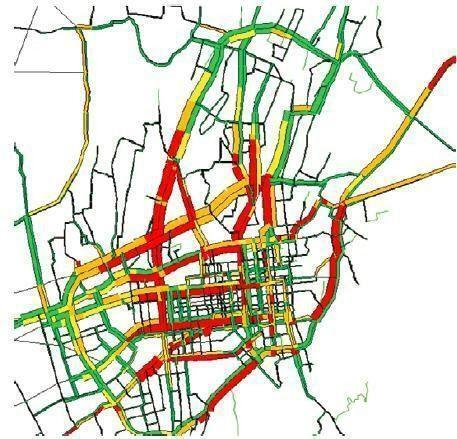
\includegraphics[width=0.6\textwidth]{assets/73}
	\caption*{Figure 1 - Forecast for 2024 of the processes of development of congestion on the central roads in the city of Almaty (overview of the current situation of congestion in Almaty according to the data yandex.kz )}
\end{figure}

\begin{multicols}{2}
The creation of collective intelligent traffic light controllers
integrated with the Scada system in an automated traffic management
system using advanced simulation of processes in the AnyLogic
environment will be a new direction in the digitalization of the
country's traffic.

The symbiosis of the two approaches creates conditions for the fruitful
modernization of existing analog traffic control systems. The phased
introduction of smart traffic lights as an IoT device will make it
possible to design and implement a modern intelligent computer network
of smart traffic light facilities that will be able to monitor the
traffic situation dynamically and allow automating optimal decisions by
dispatchers of the central traffic control panel of the megapolis
(Fig.2).
\end{multicols}

\begin{figure}[H]
	\centering
	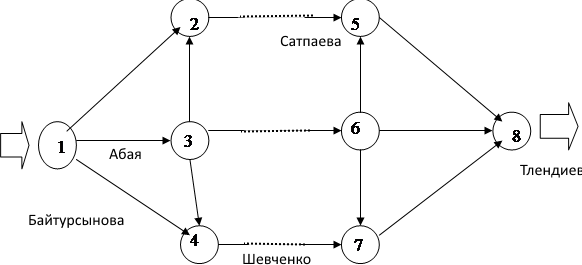
\includegraphics[width=0.5\textwidth]{assets/74}
	\caption*{Figure 2 - Graph of traffic flow during rush hour from east to west in Almaty along Abai, Satpayev and Shevchenko streets}
\end{figure}

\begin{multicols}{2}
Pilot research works on the introduction of smart traffic lights are
being carried out in the cities of Almaty and Astana. Creating a local
smart traffic light that works autonomously without taking into account
the general traffic situation can theoretically improve the throughput
on this section of road. The complexity of taking into account all
traffic parameters along urban highways during peak hours creates
prerequisites and stimulates research on the simulation of traffic
lights as the main automatic regulators of the capacity of city
highways, taking into account the multiparametric conditions of the
significantly uncertain task of optimizing car traffic on the urban road
network. The lack of a single solution devalues deterministic theories
of traffic flow management and increases the role of heuristic
(intelligent) methods for solving problems of increasing traffic in the
cities of Almaty and Astana.

One such approach is the method practiced by the Almaty City Traffic
Patrol Service to create congestion at the entrances to the city, which
reduces the load on the urban road network and creates the illusion of
orderly traffic within the city.

These contradictions create prerequisites for the introduction of
adaptive automation of traffic light cyclograms. It is really possible
to find a solution to the multiparametric problem of nonlinear automated
control of traffic light objects in a complex, taking into account
traffic jams, only on the basis of modern digital control.

To conduct the research, we used methods of systematic analysis of the
current state of traffic flow management using computer simulation
models, taking into account online geoinformation data of the temporal
and spatial position of the traffic flow as a continuum and as a
micro-participant in the traffic process. Computer technology methods
for creating network stationary and mobile digital traffic light objects
capable of identifying the traffic situation, calculating the number and
speed of traffic flow, and transmitting up-to-date data via computer
networks to a neighboring traffic light. The method of controlling a
digital smart traffic light that has an Internet connection with a
server is adaptive with feedback and with a temporary correctable
compensator.

{\bfseries The results and their discussion.} As a result of our research,
we have developed algorithms and simulation programs in the AnyLogic PL
software, taking into account the traffic situation at the entrance/exit
and in the center of Almaty city using maps of the geoinformation
system, which allow on-line dispatching services of the highway patrol
to make recommendations to the duty officers of the highway patrol
service on manual regulation of the traffic flow regime. We recommend
that the educational and research work of the country's transport
universities include methodological guidelines on simulation modeling in
the AnyLogic PLA environment in the Kazakh language. A prototype of a
collective smart traffic light based on AVR, ESP 32 and Lo@Ra chips has
been developed. Simulation models have been developed and recommended
for implementation in the AnyLogic environment for heavily trafficked
entrances/exits and the city center of Almaty, taking into account the
data of geoinformation systems.

However, despite the results achieved, there are still a number of
unresolved issues that need to be further investigated and studied.
However, the most appropriate moment to warn the driver is best checked
using a real driver and (prototype) system in real tests, since the most
appropriate moment also depends on the human factor, such as reaction
time. Therefore, in order to find the boundary values that the system
will warn about at the right moment, in practice, precise adjustment
will be required (Fig.3).

In addition, the road condition is taken into account by calculating the
braking time for a given coefficient of friction (obtained from images
on the roads). This braking time is subtracted from the braking distance
of the vehicle and used as an additional safety indicator.:
\end{multicols}

``min''
\begin{equation}
f(q) = max\left\{ \min\left\{ \frac{5 - q}{5},1 \right\},0 \right\};
\end{equation}

«zero»
\begin{equation}
f(q) = max\left\{ \min\left\{ \frac{q}{5},\frac{10 - q}{5} \right\},0 \right\};
\end{equation}

«average»
\begin{equation}
f(q) = max\left\{ \min\left\{ \frac{q - 5}{5},\frac{15 - q}{5} \right\},0 \right\};
\end{equation}

``max''
\begin{equation}
f(q) = max\left\{ \min\left\{ \frac{q - 10}{5},1 \right\},0 \right\};
\end{equation}

\begin{figure}[H]
    \centering
    \begin{subfigure}[b]{0.45\textwidth}
        \centering
        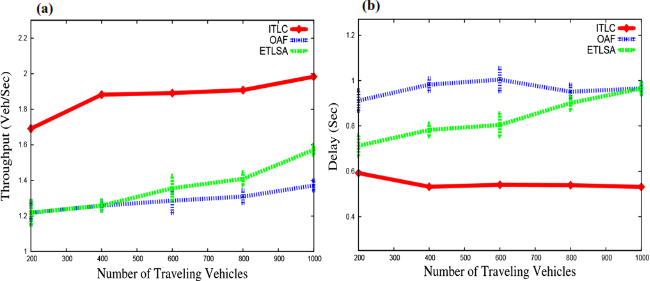
\includegraphics[width=\textwidth]{assets/75}
		\caption*{a}
    \end{subfigure}
    \hfill
    \begin{subfigure}[b]{0.45\textwidth}
        \centering
        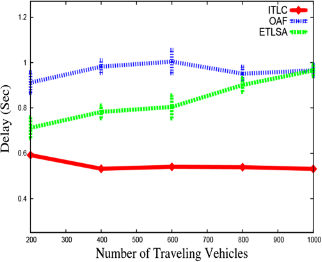
\includegraphics[width=\textwidth]{assets/75.1}
		\caption*{b}
    \end{subfigure}
\end{figure}

\begin{figure}[H]
    \centering
    \begin{subfigure}[b]{0.45\textwidth}
        \centering
        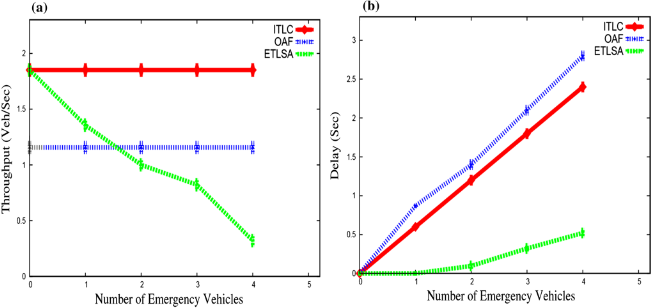
\includegraphics[width=\textwidth]{assets/76}
		\caption*{c}
    \end{subfigure}
    \hfill
    \begin{subfigure}[b]{0.45\textwidth}
        \centering
        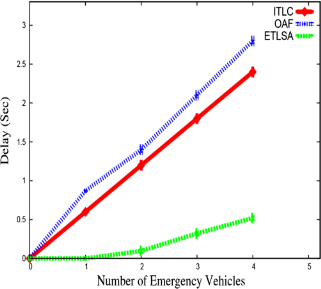
\includegraphics[width=\textwidth]{assets/76.1}
		\caption*{d}
    \end{subfigure}
	\caption*{a -- with a minimum indicator; b -- with a zero indicator; c -- with an average indicator; d -- with a maximum indicator}
	\caption*{Figure 3 - Calculation results based on a simulation model for controlling useful signals in real time}
\end{figure}

\begin{multicols}{2}
Two consecutive images of the video sequence for the intersection in
Almaty were processed in the work. This allows you to use video
recordings of the dynamics of pedestrian movement and the position of
vehicles to determine their speeds and make a forecast for the current
situation. Both video sequences were made at the rate of 25 frames per
second and were obtained from a hill from the balcony of the building.
The processing parameters (object sizes and thresholds for background
subtraction) have been configured to include pedestrians and vehicles,
but exclude lighting effects. Due to various lighting changes, for
example, due to the reflection of the sun on building windows and car
windshields, setting the parameters was a difficult task. In order to
obtain better data for the security algorithm, some stages of
preprocessing of the video sequence data sets were performed. The
preprocessing steps included:

- Track separation: If the distance between two consecutive data points
of the same object is too large, the data may be considered as belonging
to two different objects. The tracks are separated, a new identification
number is assigned to the second part of the track;

- Track connection: If the end point of one track and the start point of
another track are very close to each other in time and space, they
probably belong to the same object and have the same identification
number;

Finally, tracks of very short length (shorter than 2 meters) are not
used.

An electrical circuit for connecting this interface to the LOGO! 230RCE
microcontroller was also developed (Fig. 4).
\end{multicols}

\begin{figure}[H]
	\centering
	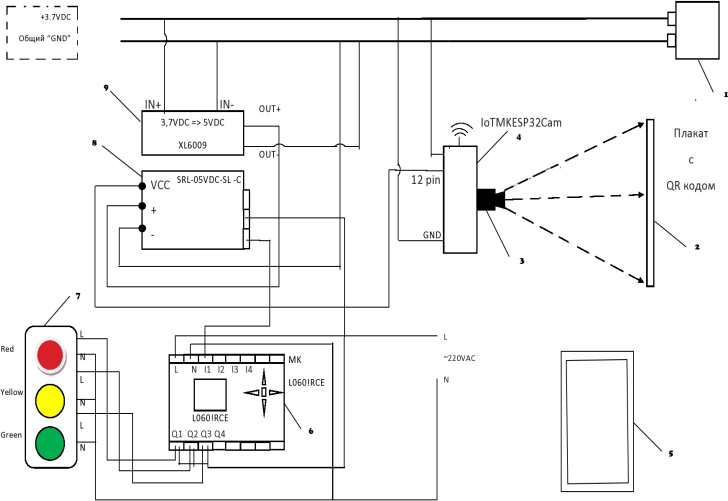
\includegraphics[width=0.8\textwidth]{assets/77}
	\caption*{1 -- ZONeSUN 18650 battery with a capacity of 3000 mAh and a
voltage of 3.7 volts; 2 -- a poster with a QR code on the windshield of
a special car; 3 -- OV 2640 webcam; 4 -- ESP32 Cam microcontroller as a
``local server''; 5 -- mobile smartphone as a ``client''; 6 --
reprogrammable traffic light microcontroller LOGO 230RCE; 7 -- traffic
light; 8 -- electromechanical relay SRL-05VDC-SL-C; 9 -- DC voltage
converter (step-up, adjustable) XL6009 from 3.7 VDC to 5 VDC}
	\caption*{Figure 4 - Electrical diagram of the smart interface for controlling a ``smart'' traffic light using a QR code}
\end{figure}

\begin{multicols}{2}
To obtain permission using the QR code displayed on a mini-poster near
the right corner of the windshield of special vehicles, it is necessary
not only to decode the code, but also to perform a number of actions
according to the requirements of the traffic rules. First, it is
necessary to recognize the information contained in the QR code in
advance. The optical system of the OV 2640 MK ESP32 Cam video camera
allows you to focus at a distance of 5-6 meters on a mini poster on the
windshield of a special car and read the data embedded in the QR code.

The controller chip must be powered with a stabilized voltage of up to
3.7 volts, but not less than 2.5 volts. Therefore, the ZONeSUN 18650
battery with a capacity of 3000 mAh was chosen as the power source. A
special feature of these power supplies is the presence of an electronic
bookmark that protects the battery from over/undercharging {[}6, 7{]}.

The supply of voltage to the ESP32 Cam microcontroller automatically
initializes the launch of the program code pre-embedded in the memory of
the smart device. After that, the MK ESP32 Cam constantly works in local
server mode, and the webcam programmatically detects the presence of a
QR code in its viewing sector.

In the case of recognition of the QR code programmed and embedded in the
memory of special machines, a voltage of up to 5 volts DC is applied to
the discrete I/O pin 12. Since the ESP32 Cam chip is a powerful current
consumer, the voltage at this pin often drops to 4.5 volts, which is not
enough to power the relay coil SRL-05VDC-SL-C. Therefore, a pull-up chip
XL6009 is connected to a common 3.7 volt DC circuit, which creates a
stabilized voltage of 5 volts at the output, powering the relay coil.

The main feature of the QR code recognition unit is the presence of a
common «GND» line. The output relay interacts with a 220 volt AC circuit
powering the LOGO! 230RCE microcontroller and traffic lights via relay
outputs Q1,Q2,Q3. The input terminal I1 receives logical information
(True) in the form of a voltage of 220 volts AC in case of recognition
of the fact of the approach of special vehicles. Thus, the standard
QRCodeReader.h program has been modified to create an intelligent
interface for a «smart» traffic light, and the created software and
hardware IoT interface has a cost of less than 10,000 tenge.

Let\textquotesingle s describe the program code for the Arduino IDE
environment, which has been adapted to these requirements. In the QR
code, for example, ambulances, a number in text form is entered, showing
the number of seconds required to cross the intersection, the \$
separator sign and the type of special car. In the case of fire trucks,
which often move in a small column, the turn-on time of the «green wave»
will be longer and this information is embedded in the QR code.

Below is a program in the Arduino IDE environment codes that implements
the adaptive green wave activation algorithm:
\end{multicols}

\begin{verbatim}
Void setup()
{
  Serial.begin(115200);
  Serial.println();
  pinMode(12,OUTPUT);
  reader.setup();
   Serial.println(“Setup QRCode Reader”);
  reader.beginOnCore(1);
Serial.println(“Begin on Core 1”);
}
void loop()
{
  if(millis() / 1000 – pastSeconds > 5){
  String code = onQrCodeText();
  int litres = ParseInt(code.substring(0, code.indexOf(‘$’)));
  String name = code.substring(code.indexOf(‘$’) + 1);
  Serial.print(“Seconds:”);
  Serial.println(seconds);
  Serial.print(“Name:”);
  Serial.println(name);
  digitalWrite(12, HIGH);
  pastSeconds = millis() / 1000;
  for(nti = 0; i < second * 2; i++){
    Serial.print(“.”);
    delay(500);
  }
  Serial.println();
  digitalWrite(12, LOW);
  code = “”;
  }
  delay(100);
}
\end{verbatim}

\begin{multicols}{2}
As can be seen from the text of the program, the webcam reads the QR
code, analyzes the text and selects a number from it, presented in text
format, and converts it into a numeric format. The smart traffic light
relay coil is then turned on to turn on the yellow light and then the
green light.

{\bfseries Conclusion.} Based on the conducted research, conclusions and
recommendations are made. The analysis of well-known patent solutions
and literature sources, new technology has shown that modern urban
traffic light facilities are the most important link in a multi-level
automated traffic management system of large cities such as Almaty and
Astana.

The studied mathematical models based on micro-macroscopic modeling of
the flow of cars are quite adequate approximations under complex and
contradictory initial and boundary conditions. Our research has also
confirmed numerous claims about the presence of oncoming logistics
traffic flows from west to east, from north to west and east, from east
to west and north to the areas of wholesale markets. The main buyers of
goods and products are residents of the city of Almaty, which leads to
massive oncoming traffic that is uneven in time of day and weeks.

It is shown that the use of modern microprocessor technology and
advances in information technology makes it possible to formalize and
automate many functions of existing analog traffic light facilities,
police officers, environmentalists and traffic controllers. Automation
and intellectualization of the performance of a number of regulatory
functions of traffic management corresponds to modern trends in the
development of a digital society in the context of the Modernization 4.0
concept.
\end{multicols}

\begin{center}
{\bfseries References}
\end{center}

\begin{noparindent}
1.Badaguev B.T. Jekspluatacija transportnyh sredstv (organizacija i
bezopasnost\textquotesingle{} dvizhenija).- M.:
Al\textquotesingle fa-Press, 2019. - 239 s. ISBN: 978-5-64280-556-2
{[}in Russian{]}

2.Dudko N.I., Petrovec V.R., Bershadskij V.F.
Bezopasnost\textquotesingle{} dvizhenija mehanicheskih transportnyh
sredstv.-Gorki: BGSHA, 2014.- 238 c. ISBN: 978-985-467-490-2. {[}in
Russian{]}

3. Bershadskij V.F., Dudko N.I. Bezopasnost\textquotesingle{} dorozhnogo
dvizhenija. -- Minsk: Uradzhaj, 1990. -- 271 s. ISBN: 5-7860-0004-4.
{[}in Russian{]}

4.Blinkin M.Ja. Bezopasnost\textquotesingle{} dorozhnogo dvizhenija:
istorija voprosa, mezhdunarodnyj opyt, bazovye institucii. -M.: Izd. dom
Vysshej shkoly jekonomiki, 2013. -- 240 c. ISBN: 978-5-7598-1086-5.
{[}in Russian{]}

5.Volkov V.S. Jelektrooborudovanie transportnyh i
transportno-tehnologicheskih mashin: ucheb. pos. -- M.:

Akademija, 2010.
-- 208 s. ISBN: 9785769557491.{[}in Russian{]}

6.Gorev, A. Je. Osnovy teorii transportnyh sistem: ucheb. posobie / A.
Je. Gorev; SPbGASU. -- SPb., 2010.- 214 s. ISBN: 978-5-9227-0266-9.
{[}in Russian{]}

7.Bednarskij V.V.,Majboroda M.E., Gruzovye avtomobil\textquotesingle nye
perevozki. -- M.: Feniks, 2008. - 442 s. ISBN:978-5-222-11805-4. {[}in
Russian{]}
\end{noparindent}

\emph{{\bfseries Information about authors}}

\begin{noparindent}
Tulegulov А. D.- Candidate of Physical and Mathematical Sciences, аss.
professor, K.Kulazhanov Kazakh University of Technology and Business,
Astana, Kazakhstan, е-mail: tad62@ya.ru;

Akishev K.M.- Candidate of Technical Sciences, ass. professor, K.
Kulazhanov Kazakh University of Technology and Business, Astana,
Kazakhstan,e-mail: akmail04@mail.ru;

Zhamangarin D.S.- PhD, аssociate professor, K. Kulazhanov Kazakh
University of Technology and Business, Astana, Kazakhstan, е-mail:
Dus\_man89@mail.ru;

Sataev B. O.- Candidate of Technical Sciences, ass. professor.
Kulazhanov Kazakh University of Technology and Business, Astana,
Kazakhstan, е-mail: sbo@mail.ru.
\end{noparindent}

\emph{{\bfseries Сведение об авторах}}

\begin{noparindent}
Тулегулов А.Д.-к.ф.-м.н., асс. профессор, Казахский университет
технологии и бизнеса им. К. Кулажанова, Астана. Казахстан, е-mail:
tad62@ya.ru;

Акишев К. М.-к.т.н., асс. профессор,Казахский университет технологии и
бизнеса им. К. Кулажанова, Астана, Казахстан, е-mail: akmail04@mail.ru;

Жамангарин Д.С.- PhD, асс. профессор, Казахский университет технологии и
бизнеса им. К. Кулажанова, Астана, Казахстан,е-mail: Dus\_man89@mail.ru;

Сатаев Б.О.-к.т.н., асс. профессор, Казахский университет технологии и
бизнеса им. К.Кулажанова, Астана, Казахстан,е-mail: sbo@mail.ru.
\end{noparindent}
